\chapter{Wprowadzenie}

\section{Wstęp}


\section{Ataki rekonesansowe}
Ataki rekonesansowe są typem ataków komputerowych, których głównym celem jest pozyskanie informacji na temat atakowanego systemu bądź
podatności, które w nim występują. Słowo ,,rekonesans'' zostało zapożyczone z nomenklatury militarnej i odnosi się do zapoznania z
terenem wroga. W kontekście ataków na sieci komputerowe stwierdzeniem określa się analogiczny krok -- działanie przed właściwym atakiem.
Sam rekonesans można podzielić dodatkowo na dwie kategorie: atak aktywny oraz pasywny.
Atak aktywny odnosi się do działania, gdy atakujący podejmuje akcje, przez które może wchodzić w interakcję z systemem, na przykład
wysyłanie specjalnie spreparowanych zapytań czy skanowanie portów.

Atak pasywny to tylko i wyłącznie obserwacje działającego systemu. Może to być na przykład podsłuchiwanie ruchu, analiza najczęściej
odwiedzanych stron, czy choćby przyglądanie się innym procesom aby odpowiednio przygotować atak właściwy.

Obie wersje ataków rekonesansowych są również częścią tak zwanego etycznego hakowania (ang. \textit{ethical hacking}). Osoby które
tym się zajmują (określani po angielsku jako \textit{white hat}) starają się wytknąć błędy i podatności w systemach przy czym starają
się nie ingerować w ich działanie.

Innym podziałem, który pojawia się w kontekście ataków rekonesansowych, jest podział na 4 grupy. Każda z nich określa atak
przeprowadzany w innych warunkach, środowisku. Zaproponowany podział uwzględnia nie tylko techniczne aspekty pozyskiwania informacji
o systemie, ale również kwestie społeczne, jak na przykład próby uzyskania danych od pracowników firm, bądź ogólnie użytkowników
systemów. Kompletną listę grup wyróżnionych w tym podziale zaprezentowano oraz krótko opisano w tabeli \ref{tab:rekonesans}.

\begin{longtable}{|c|p{4cm}|p{8cm}|}

	\hline
	\textbf{Lp.} &
	\textbf{Obszar pozyskiwania informacji} &
	\textbf{Opis} \\ \hline\hline
	1 & Profil sieci &
	Pozyskiwanie informacji na temat infrastruktury sieciowej: adresy IP, domeny, poddomeny; informacje na temat topologii
	systemu.\\
	\hline
  	2 & Profil środowiska &
	Pozyskiwanie informacji na temat przypadków użycia systemu, aktorów, grup, nazw użytkowników, wykorzystanego sprzętu, architektury,
	portów na których uruchomione są usługi.
  	\\
	\hline
	3 & Profil użytkowników systemu &
	Informacje ,,społeczne'' -- imiona, nazwiska, numery telefonów, plotki, określenie poziomu wiedzy na temat systemów
	telekomunikacyjnych, informatycznych, zabezpieczeń.
	\\
	\hline
	4 & Profil zabezpieczeń &
	Określenie poziomu, profilu zabezpieczeń fizycznych (np. konroli dostępu), złożoności haseł wymaganych przez system, pozyskanie
	informacji na temat systemów wykrywania włamań.\\
	\hline
	\capiton{Typy rekonesansu, opis na podstawie \cite{rekonesans}}
	\label{tab:rekonesans}
\end{longtable}

Z uwagi na techniczny charakter niniejszej pracy magisterskiej w kolejnych rozdziałach skupiono się głównie na rekonesansie odnoszącym
się do infrastruktury systemów. Mowa tu zarówno o infrastrukturze sieciowej jak i profilu sprzętowym odpytywanych maszyn. Ataki tego typu
są najczęsciej przeprowadzane poprzez wykonanie kilku testów, jednak nie są to jedyne sposoby pozyskiwania informacji o infrastrukturze.
Jednym z podstawowych, powszechnie spotykanych przykładów aktywnego rekonesansu jest skanowanie portów. Proces ten jest zaliczany
do ataku aktywnego, ponieważ atakujący próbuje dowiedzieć się, na których portach danego systemu uruchomione są usługi (np. FTP, www,
serwer pocztowy, SSH). Uzyskanie takich danych pozwala w późniejszym etapie na wykorzystanie podatności danych usług, wynikających
głównie z błędnej implementacji bądź konfiguracji. Prowadzi to następnie do eskalacji uprawnień na maszynie na rzecz atakującego.
Przykładowe wykorzytanie danych podatności na podstawie usługi SSH opisane zostało w dokumencie \cite{ssh_podatnosci}.

Inną formą rekonesansu dotyczącego infrastruktury systemu jest rekonesans DNS. Jest to część testu penetracyjnego polegającą na pozyskaniu jak największej ilości informacji na temat badanej domeny.
Dane uzyskiwane podczas jego przeprowadzania odnoszą się zarówno do serwera DNS jak i wpisów, które przechowuje. Zebrane informacje mogą
kompromitować infrastrukturę sieciową firmy nie powodując przy tym generowania zbyt podejrzanego ruchu. Między innymi dlatego
ważne jest, aby przywiązywać znaczną uwagę do tego kto i w jaki sposób próbuje łączyć się z serwerami autorytatywnymi odpowiedzialnymi
za domenę. W sytuacji, gdy badana jest jedna domena, bądź zbiór kilku domen pod zarządem jednej organizacji wykorzystywane są najczęściej
narzędzia dostępne w różnego rodzaju pakietach, na przykłąd BIND \cite{isc}. Przykładami takich programów są dig \cite{dig} czy
nslookup \cite{domain_example}. Oba pozwalają na wysyłanie zapytań DNS do serwerów. Największą zaletą wspomnianych narzędzi jest
możliwość dostosowywania pól w wiadomościach do potrzeb użytkownika. Dodatkowo nslookup umożliwia również pracę w trybie serwera,
jednak bardziej istotna dla atakujących jest sama generacja zapytań, dzięki którym można uzyskać informację na temat testowanego
systemu.

Jednym z największych błędów, które można popełnić przy konfiguracji serwera DNS jest umożliwienie przeprowadzenia transferu strefy
DNS przez nieautoryzowane serwery. Jest to istotna kwestia dla każdego z serwerów do których można kierować zapytania z sieci zewnętrznej.
W takim przypadku atakujący otrzymuje informacje o całej strefie przechowywanej na serwerze. Problem ten staje się jeszcze bardziej
poważny w momencie, gdy serwer DNS obsługuje zarówno sieć wewnętrzną jak i zewnętrzną. Ujawnienie danych systemu DNS sieci
wewnętrznej jest równoznaczny z udostępnieniem planu sieci, która jest przez niego obsługiwana.


AXFR (\textit{ang. Asynchronous Xfer Full Range}) \cite{RFC1034, RFC1035} to mechanizm używany w protokole DNS (\textit{Domain Name System}) do
transferowania strefy, za którą odpowiada serwer nazw. Głównym przeznaczeniem opisywanego standardu był transfer informacji pomiędzy
podstawowym i zapasowym serwerem przestrzeni nazw. Zasada jego działania jest bardzo prosta -- serwer podrzędny (\textit{ang. slave})
przesyła żądanie AXFR do serwera podstawowego (\textit{ang. primary, master}).

Oczywiste jest, że AXFR jest wykorzystywany w celach zupełnie innych niż te, do których go zaprojektowano. Mowa tu o sytuacji,
w której serwer główny w żaden sposób nie weryfikuje po swojej stronie źródła takiego zapytania. Prowadzi to do sytuacji, w której
każdy, kto jest w stanie utworzyć odpowiedni pakiet TCP może wejść w posiadanie informacji o całej strefie, za którą odpowiada
odpytywany serwer DNS. Wspomniane przygotowanie pakietu DNS nie jest specjalnie trudne, ponieważ umożliwia to wiele narzędzi, na
przykład dig \cite{dig}, wchodzący w skład pakietu bind \cite{isc}.

\section{Domain Name System}
Głównym zadaniem protokołu DNS (\textit{Domain Name System}) \cite{RFC1035} jest translacja nazw przyswajalnych dla użytkowników (najczęściej
alfanumerycznych) na nazwy sieciowe, czyli adresy IP.

DNS jest jednym z podstawowych elementów internetu. Z wystawionego przez niego interfejsu korzysta wiele usług sieciowych i innych
protokołów. Można traktować go jako bazę danych, która jest rozproszona po wielu lokalizacjach. Ponadto, system powinien oraz
cechuje się dużą niezawodnością. W tym przypadku została ona osiągnięta poprzez wprowadzenie dość prostego mechanizmu -- nadmiarowości
serwerów. To właśnie dzięki tej redundancji DNS cechuje się wysokim wskaźnikiem niezawodności, gdyż w momencie gdy któryś z serwerów
nie odpowiada informacja pobierana jest z innego serwera -- zapasowego, podrzędnego.

System DNS ma charakterystyczną, hierarchiczną strukturę, którą zaprezentowano na rysunku \ref{hierarchy_dns}. Na rysunku
przedstawiono węzeł główny (ang. \textit{root}) reprezentowany jako znak pojedynczej kropki oraz przykład dwóch typów domen
pierwszego poziomu.

\begin{center}
	\begin{figure}
	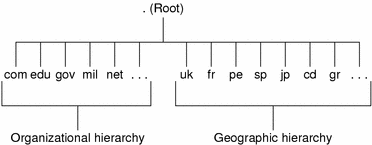
\includegraphics[scale=1]{image/hierarchy_dns}
	\caption{Heriarchia systemu DNS \cite{hierarchy_dns}.}
	\label{hierarchy_dns}
	\end{figure}
\end{center}

Dzięki tej hierarchii systemu możemy powiedzieć o DNS, że charakteryzuje go bardzo dobra skalowalność oraz elastyczność.

Podział ze względu na położenie geograficzne jest oczywiście bardziej naturalny i łatwy zarówno do wdrożenia jak i zrozumienia.
Każdemu z państw przydzielono dwuliterowy identyfikator, który reprezentuje domenę najwyższego poziomu odpowiadającą
danemu państwu. Dozwolone są także trzyliterowe identyfikatory domen najwyższego poziomu (np com, net, org), które z reguły
przypisywane są różnego rodzaju organizacjom. Powołując się na informacje przedstawione na grafice \ref{hierarchy_dns}
TLD o identyfikatorze \textit{uk} odpowiada domenom utożsamianym z Wielką Brytanią, a \textit{fr} -- domenom francuskim.

Hierarchia systemu DNS wynika z faktu, że domenami internetowymi każdego poziomu może zarządzać inna organizacja. Odnosi się to
zarówno do domeny \textit{root}, jak i domen najwyższego poziomu niezależnie od przynależności grupowej. W Polsce identyfikatorem
TLD jest sufiks \textit{pl}, a jednostką odpowiedzialną za nią jest CERT Polska \cite{cert}. Jeśli użytkownik chciałby dołączyć
ze swoją siecią do internetu powinien zgłosić do odpowiedniej organizacji taką chęć oraz dostarczyć wszystkich niezbędnych
informacji, które są wymagane przez zarządcę.

Bardzo ważnym punktem jest wspomniana w poprzednim akapicie ,,chęć'' dołączenia do internetu. Jeśli użytkownik czy organizacja
chcą używać protokołu DNS jedynie do użytku wewnętrznego, to nie ma restrykcyjnych ograniczeń co do używanych nazw. Jeśli natomiast
oczekuje się wystawienia domen w taki sposób, aby były widoczne z zewnątrz, to należy odpowiednio:
\begin{enumerate}
	\item zarejestrować nazwę domeny,
	\item pozyskać adres IP.
\end{enumerate}

Bardzo trafne jest tu porównanie całego systemu Domain Name System do struktury plików w systemach operacyjnych z rodziny UNIX.
Nazwa domeny bezpośrednio określa jej miejsce w całej przestrzeni nazw, podobnie jak ścieżka bezwzględna pliku określa jego miejsce
w całym systemie plików. Po rejestracji domeny, jest ona dołączana w odpowiednie miejsce w hierarchii. Przykład domeny \textit{google.com}
razem z jej poddomenami i odpowiednimi miejscami w hierarchii systemu przedstawiono na rysunku \ref{example_domain_tree}.

\begin{center}
	\begin{figure}
	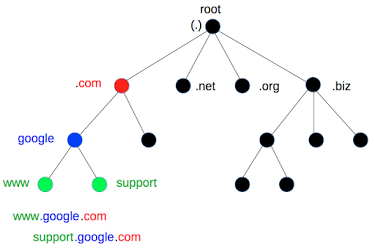
\includegraphics[scale=1]{image/domain_tree}
	\caption{Położenie domeny w przestrzeni nazw \cite{domain_tree_src}.}
	\label{example_domain_tree}
	\end{figure}
\end{center}

Serwer autorytatywny (ang. \textit{authoritative name server}) posiada odgórne przyzwolenie na zarządzanie nazwami swoich hostów
(kto przyznaje(?) \cite{toDoWarning}). Ze względu na drzewiastą strukturę systemu można oczekiwać, że kolejne domeny oraz ich serwery
autorytatywne będą delegować odpowiedzialność za kolejne strefy do serwerów niższego poziomu. W ten sposób, powołując się na przykład
przedstawiony na rysunku \ref{example_domain_tree} serwer autorytatywny .com zarządza nazwami w domenie .com, natomiast zarządzanie
nazwami w domenie google.com przekazuje do niższego szczeblem serwera przestrzeni nazw. W ten sposób serwer domeny google.com ma
możliwość przypisywania nazw takim domenom jak zaprezentowane support.google.com.

\subsection{Podział domen najwyższego poziomu}
Jeśli chodzi o podział domen pierwszego poziomu ze względu na przynależność organizacyjną, to aktualny stan przedstawiony jest w
tabeli poniżej.

\begin{table}[]
	\centering
	\caption{Podział domen najwyższego poziomu ze względu na działalność.}
	\label{podzial_tld}
	\begin{tabular}{|r|p{10.5cm}|}
		\hline
		\textbf{TLD} & \textbf{Opis jednostki} \\
		\hline\hline
		com & Jednostki o działalności komercyjnej (ang. \textit{commercial institutions}) \\
		\hline
		edu & Jednostki edukacyjne (ang. \textit{educational institutions})\\
		\hline
		gov & Instytucje rządowe (ang. \textit{government institutions}) \\
		\hline
		mil & Grupy wojskowe (ang. \textit{military groupos}) \\
		\hline
		net & grupy związane z działaniem sieci (ang. \textit{network support centers}) \\
		\hline
		org & Organizacje nonprofit i inne (ang. \textit{nonprofit organizations}) \\
		\hline
		int & Organizacje międzynarodowe (ang. \textit{international organizations}) \\
		\hline
	\end{tabular}
\end{table}

Przedstawiony podział nie jest stały. Autorzy zastrzegli, że w przyszłości może być on rozszerzony o dodatkowe kategorie.

\subsection{Domena DNS}
Domeną określa się dany podzbiór hierarchii DNS. Są to wszystkie poddomeny podlegające tej samej domenie wyższego poziomu. Odnosząc
się do wcześniej przywołanego porównania do systemu plików -- domena to odpowiednik folderu. Może zawierać kolejne domeny, może być
określana zarówno na bardzo wysokim (domeny poziomu TLD) jak i bardzo szczegółowym (domeny 2-3 LD) poziomie abstrakcji. Jeśli
chcielibyśmy reprezentować system DNS jako drzewo, to domeną DNS nazwiemy węzeł drzewa i wszystkie węzły, które są jego potomkami.
Pojęcie domeny i elementy, które ono określa przedstawiono na rysunku \ref{fig:domain_dns_example}.

\begin{center}
	\begin{figure}
	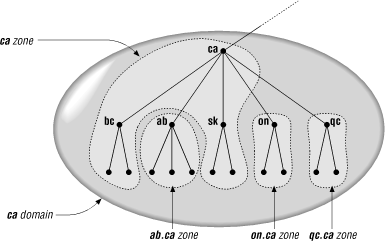
\includegraphics[scale=0.8]{image/domain_example}
	\caption{Zakres drzewa hierarchii DNS wchodzący w skład domeny \cite{domain_example}.}
	\label{fig:domain_dns_example}
	\end{figure}
\end{center}

\subsection{Strefa DNS}
Strefa DNS jest pojęciem, które określa zbiór domen, za które odpowiedzialny jest konkretny serwer przestrzeni nazw. Jeśli wyobrazimy
sobie hierarchię DNS jako drzewo, w którym węzłami są kolejne nazwy domen, to strefą DNS będzie zbiór węzłów tego drzewa. Zbiór
węzłów wyznaczany jest na podstawie informacji o serwerze autorytatywnym odpowiedzialnym za daną domenę. Te węzły (domeny)
których nazwami zarządza ten sam serwer znajdują się w jednej strefie DNS. Przykładowy podział systemu na konkretne strefy został
zaprezentowany na rysunku \ref{fig:dns_zone_example}.

\begin{center}
	\begin{figure}
	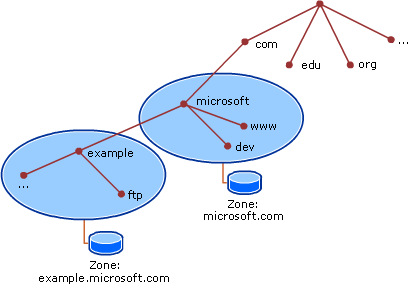
\includegraphics[scale=0.8]{image/zone_example}
	\caption{Zakres drzewa DNS określany terminem strefy DNS \cite{zone_example}.}
	\label{fig:dns_zone_example}
	\end{figure}
\end{center}

\subsection{Strefa DNS a domena DNS}
System DNS danej domeny jest zrealizowany w oparciu o zbiór serwerów przestrzeni nazw (ang. \textit{nameserver}). Każdy z serwerów
może być serwerem autorytatywnym dla pojedynczej domeny, wielu domen bądź domen wraz z odpowiadającymi im poddomenami. Wycinek
przestrzeni zarządzany przez określony serwer nazywany jest strefą DNS.


\subsection{Kompletne nazwy domen}
\label{sec:FQDN}
Określeniem pełne, kompletne lub zupełne nazwy domen (ang. \textit{Fully Qualified Domain Names (FQDNs)}) nazywane są te domeny,
których nazwy zawierają domenę każdego poziomu, począwszy od lokalnej, aż po domenę główną, czyli root. Łatwo dostrzec analogię
do wcześniej wspomnianego systemu pliku w systemach operacyjnych UNIX pomiędzy FQDN a bezpośrednią ścieżką do pliku. Różnicą jest
tu jednak sposób odczytywania takiej ścieżki. W systemach DNS najbardziej ogólny węzeł znajduje się na skrajnie prawej pozycji a
poruszając się w stronę lewą dochodzimy do kolejnych lokalnych domen.

\subsection{Mapowanie nazw na adres IP}
\label{mapping}
Mapowanie nazw domeny na jej adres IP jest możliwe dzięki plikom strefy DNS, które znajdują się na autorytatywnym serwerze
przestrzeni nazw, tzw. \textit{zone files}. Jeden z typów tych plików przechowuje nazwy domen wraz z odpowiadającymi im adresami
IP. Gdy klient chce dowiedzieć się pod jaki adres kierować swoje zapytanie, kieruje informacje do serwera autorytatywnego. On
odpowiada za znalezienie i przedstawienie mapowania nazwy na adres IP, dokonując przeszukania plików strefy.

\subsection{Mapowanie odwrotne}
\label{revmapping}
Baza danych DNS może także zawierać pliki, które umożliwiają mapowania odwrotne, tj. adresu IP na nazwę domeny/hosta. Mechanizm ten
może być użyty przy próbie weryfikacji pochodzenia wiadomości. Chcąc wykluczyć próbę oszustwa ze strony prawdziwego nadawcy możemy
posiłkować się właśnie odwrotnym mapowaniem. Możemy zweryfikować, czy adres IP mapowania odwrotnego zgadza się z adresem IP z którego
nadano wiadomość. Mechanizm ten może być również wykorzystywany do autoryzacji operacji wykonywanych zdalnie.

Odwrotne mapowanie wykorzystuje specjalną domenę \textit{in-addr.arpa}. Z założenia domena ta wykorzystuje adresy IP zamiast adresów
domen.  Wspomniana domena jest częścią strefy DNS, która umożliwia takie właśnie odwzorowanie. Istotne jest, że adresy w domenie
\textit{in-addr.arpa} są zapisywane w specyficzny dla siebie sposób -- od najniższego do najbardziej istotnego poziomu. Wynika z
tego, że adresy IP w opisywanej domenie są w pewnym sensie zapisywane ,,od końca''. Powołując się na przykład, załóżmy, że maszyna
ma przypisany adres 10.8.0.32. W plikach strefy dla domeny in-addr.arpa adres ten będzie zapisany jako 32.0.8.10.in-addr.arpa.
oczywiście z kropką po członie \textit{in-addr.arpa}, która reprezentuje domenę \textit{root}.

\subsection{Wpisy plików strefy}
Tak jak wspomniano we wcześniejszych punktach \ref{mapping} oraz \ref{revmapping} działanie całego mechanizmu mapowana (czy to
właściwego czy odwrotnego) może zachodzić dzięki serwerom autorytatywnym oraz przechowywanym przez nie plikom strefy DNS.

Z racji, że system DNS dostarcza administratorom wielu funkcji poza standardowym mapowaniem adresów na IP, wpisy w bazach danych
mogą być różnych typów. Najpopularniejsze typy to oczywiście te, z którymi można zetknąć się każdego dnia, na przykład wpis typu
\textit{A} -- tłumaczący nazwę hosta na adres IP w wersji 4, \textit{AAAA} -- mapujący nazwę hosta na adres IP w wersji 6, rekordy
\textit{CNAME} służące do aliasów, czy MX -- specyfikujące serwer wymiany wiadomości elektronicznych dla danej domeny. Oprócz
wspomnianych podstawowych typów twórcy standardu dla systemu DNS wprowadzili także mniej znane typy. Opis zbioru najbardziej
istotnych wpisów określonych w dokumencie RFC 1035 \cite{RFC1035} wraz z ich przeznaczeniem umieszczono w tabeli \ref{typyRekordowDns}.

\begin{longtable}{|l|p{3cm}|p{8cm}|}

	\hline
	\textbf{Rekord} &
	\textbf{Pełna nazwa} &
	\textbf{Pełniona funkcja(opis zawartości)} \\ \hline\hline
	A &
	Wpis mapowania adresów (ang. \textit{Address mapping record}) &
	Określa adres IP wersji 4 dla danego hosta. Służą do konwersji nazwy domen do odpowiednich adresów IP.\\
	\hline
	CNAME &
	Nazwa kanoniczna (ang. \textit{Canonical Name)} &
	Określa alias. Ruch kierowany do domeny o takiej nazwie przekierowywany jest do domeny wyspecyfikowanej
	w rekordzie CNAME.
	\\
	\hline
	MX &
	Wymiana wiadomości elektronicznych (ang. \textit{Mail exchange)} &
	Na podstawie nazwy domeny znajdującej się w adresie poczty wskazuje serwer poczty elektronicznej, który odpowiedzialny jest
	za przyjmowanie tych wiadomości. We wpisie znajduje się również priorytet używany wówczas, gdy dostępnych jest więcej serwerów
	pocztowych. Ponadto, zbiór rekordów w domenie wykorzystywany jest do trasowania wiadomości w protokole SMTP.
	\\
	\hline
	NS &
	Serwer nazw (ang. \textit{Name server)} &
	Określa nazwę serwera, który został oddelegowany do obsługi danej domeny.
	\\
	\hline
	SOA &
	Wskaźnik na początkowy węzeł hierarchii (ang. \textit{Start of Authority)} &
	Wpis SOA zawiera informacje dotyczące zarządzania strefą. Jest istotny głównie z punktu widzenia transferu strefy DNS.
	Składa się z odpowiednich wpisów:
	\begin{itemize}
		\item primary -- adres serwera głównego (ang. \textit{primary}) dla danej strefy,
		\item adres poczty administratora,
		\item numer seryjny -- uaktualniany przy każdej zmianie informacji w pliku strefy,
		\item czas życia -- czas w sekundach określający okres odpytywania serwera głównego przez serwer podrzędny o numer seryjny pliku strefy; zapewnia spójność danych na serwerach podrzędnych,
		\item ponowienie żądania -- czas, który powinien odczekać serwer podrzędny jeśli serwer główny nie odpowiedział na żądanie (w sekundach); po jego upłynięciu możliwe jest ponowne wysłanie żądania,
		\item czas przedawnienia -- czas w sekundach, po którym serwer podrzędny powinien przestać odpytywać serwer podstawowy,
		\item TTL czas przechowywania odpowiedzi typu NXDOMAIN od serwera autorytatywnego (ang. \textit{negative caching}).
	\end{itemize}
	\\
	\hline
	TXT &
	Tekst &
	Wpis przeznaczony do umieszczania dodatkowych informacji dla klienta. Jest to niesformatowany tekst, może być informacją
	zarówno dla człowieka jak i maszyny.\\
	\hline
	\caption{Rodzaje rekordów w bazach danych serwerów przestrzeni nazw. Opis na podstawie \cite{RFC1035}.}
	\label{typyRekordowDns}
\end{longtable}

Oczywiście na przestrzeni lat protokół rozszerzano o kolejne funkcje. Jednym z istotnych wydarzeń było zaproponowanie zmian
spisanych w dokumencie RFC 4034 \cite{RFC4034}. Opisano tam rozszerzenia protokołu DNS, które podnoszą jego bezpieczeństwo.
W tabeli \ref{typyRekordowDnsExt} przedstawiono najważniejsze z punktu widzenia niniejszej pracy typy rekordów, które zostały
wprowadzone w kolejnych dokumentach RFC, których dokładne numery zostały wspomniane przy konkretnych wpisach w tabeli.

\begin{table}[]
	\centering
	\caption{Rodzaje rekordów w bazach danych serwerów przestrzeni nazw określonych w rozszerzeniach dokumentu RFC 1035 \cite{RFC1035}.}
	\label{typyRekordowDnsExt}
	\begin{tabular}{|r|p{3cm}|p{8cm}|}
		\hline
		\textbf{Rekord} &
		\textbf{Pełna nazwa} &
		\textbf{Pełniona funkcja(opis zawartości)} \\
		\hline\hline
			AAAA &
			Wpis mapowania adresów IPv6 &
			Określa adres IP wersji 6 dla danego hosta. Zasada działania jest taka jak w przypadku rekordu A z jedyną różnicą
			w wersji adresu IP. \\
		\hline
	\end{tabular}
\end{table}

\subsection{TLD ARPA}
Specyficzną domeną najwyższego rzędu jest domena \textit{ARPA}. Jest to jedna z nielicznych domen ściśle powiązana z dokładnie jedną
instytucją. Skrót ARPA wywodzi się historycznie od nazwy jednostki (ang. \textit{Advanced Research Projects Agency (ARPA)}), która
brała czynny udział w propagowaniu oraz rozwijaniu sieci Internet. Dzięki tej jednostce powstał między innymi prekursor dzisiejszego
Internetu -- ARPANET. Aktualnie TLD ARPA jest wykorzystywane jedynie w celach dotykających infrastruktury internetu. Skrót rozwijany jest
jako Address and Routing Parameter Area.

Tę domenę wykorzystuje się również w przypadku protokołu RevDNS a konkretniej do tłumaczenia
odwrotnego adresów IP na nazwy domen. Każdy z adresów znajduje się w poddomenie .arpa. Są to odpowiednio poddomeny in-addr.arpa dla
adresów IPv4 oraz ip6.arpa dla adresów IPv6.

Innym z zastosowań domeny .arpa jest mapowanie numerów telefonów. Sposób integracji sieci Internet wraz z siecią telefoniczną również
wykorzystuje zalety systemu DNS oraz pozwala na identyfikację odpowiednich przestrzeni nazw. Aby odróżnić przestrzeń nazw sieci
Internet od sieci telefonicznej wydzielona została domena drugiego poziomu w TLD arpa. Otrzymała ona nazwę e164. Mechanizm mapowania
numerów tradycyjnej sieci
PSTN na adresy internetowe ma szczególne znaczenie w integracji dwóch technik wykonywania połączenia, a konkretnie PSTN oraz VoIP.
Mapowanie numerów na adresy internetowe zostało opisane między innymi w RFC3761 \cite{RFC3761}.

\subsection{Plik strefy DNS}
Strefy DNS są przechowywane na serwerach w formie specjalnie sformatowanych plików. To w nich definiuje się oraz umieszcza kolejne
wpisy, rekordy, które będą zwracane dla różnego rodzaju zapytań. Plik strefy jest jednym z kluczowych jeśli chodzi o konfigurację
serwera DNS. Na listingu \ref{list:dns_zone_file} zaprezentowano przykładowy plik strefy DNS wraz z kilkoma wpisami. Przedstawiony
plik jest zformatowany zgodnie z wymaganiami stawianymi przez implementację serwera DNS zawartą w pakiecie
BIND \cite{Liu:2006:DB:1197828, isc, domain_example}.

\begin{lstlisting}[label={list:dns_zone_file},captionpos=b,caption=Przykładowy plik strefy DNS.,language=bash]
	$TTL 2d
	$ORIGIN example.com.
	@              IN      SOA   ns1.example.com. hostmaster.example.com. (
	               2003080800
	               2h
	               15M
	               3W12h
	               2h20M
	               )
	              IN      NS     ns1.example.com.
	              IN      NS     ns2.example.com.
	              IN      MX     10 mail.example.com.
	ns1           IN      A      192.168.0.3
	ns2           IN      A      192.168.0.4
	mail          IN      A      192.168.0.5

	$ORIGIN us.example.com.
	@             IN      NS     ns3.us.example.com.
	              IN      NS     ns1.example.com.
	ns3           IN      A      10.10.0.24
	$
\end{lstlisting}

Na listingu \ref{list:dns_zone_file} zaprezentowano definicję domeny \textit{example.com} oraz poddomeny \textit{us.example.com}.
Plik rozpoczyna się od definicji czasu aktywności każdego z rekordów (linia 1), który wynosi 2 dni. Kolejnym poleceniem jest
wskazanie dla jakiej domeny definiowane są wpisy DNS. Pierwszym wpisem jest rekord SOA. Kolejne pola zawarte w tym rekordzie
zostały już opisane w tabeli \ref{typyRekordowDns}. Kolejne wpisy (linie 10 oraz 11) dostarczają informacji o serwerach przestrzeni
nazw, które obsługują daną domenę. Następnie umieszczona jest informacja o głównym serwerze pocztowym w domenie. Linie 13--15
zawierają informację o adresach IP przypisanych do usług zdefiniowanych w poprzednich rekordach DNS. Są to odpowiednio dwa serwery
przestrzeni nazw (ns1 oraz ns2) oraz jeden serwer poczty elektronicznej (mail).

W linii 17 zapoczątkowana została kolejna logiczna część pliku strefy. Jest to początek definiowania wpisów dla domeny
\textit{us.example.com} czyli domeny niższego poziomu wcześniej zdefiniowanej \textit{example.com}. Zaprezentowany przypadek jest
przykładem delegacji odpowiedzialności za translację nazw do innego serwera DNS. Jest to zrealizowane poprzez umieszczenie wpisu
\textit{IN NS ns3.us.example.com}. Informuje on o tym, że serwerem przestrzeni nazw w danej poddomenie jest serwer z prefiksem
\textit{ns3}. Dodatkowo umieszczono również informację o serwerze dla domeny wyższego poziomu (\textit{ns1}). Ostatni rekord
zaprezentowany na listingu wskazuje adres IP wersji 4. wypunktowanego wcześniej serwera \textit{ns3}.

Zaprezentowana notacja jest tylko jedną z kilku, których można użyć do definiowania plików strefy DNS. W przypadku pakietu BIND
istotne jest, że fraza \$ORIGIN <domena> obowiązuje od miejsca, gdzie została użyta aż do kolejnej definicji domeny bądź do końca
pliku.


\section{Transfer strefy DNS}
Transfer strefy DNS jest typem transakcji DNS, która jest podstawowym elementem mechanizmu odtwarzania bazy danych DNS pomiędzy
serwerami systemu. Transfer jako protokołu warstwy 4 używa TCP i przybiera formę komunikacji typu klient-serwer. Zgodnie z założeniem
projektantów klient jest podrzędnym lub zapasowym serwerem DNS a serwer, który odpytuje to nadrzędny bądź główny serwer DNS. To, co
wysyłane jest w odpowiedzi od serwera głównego jest strefą DNS -- część bazy danych przechowywanych na głównym serwerze.

Transfer może odbywać się za pośrednictwem dwóch wyspecyfikowanych rodzajów zapytań -- AXFR \cite{RFC1034, RFC5936} bądź
IXFR \cite{RFC1995}. To pierwsze definiuje transfer całej strefy, niezależnie od jej wersji czy zmian które zostały naniesione,
zaś drugie transfer ,,inkrementalny'' czyli na podstawie informacji zawartych w otrzymanym zapytaniu klienckim potrafi wydzielić
tylko tę część strefy, która się zmieniła i przesłać tylko te rekordy w odpowiedzi.

Niezależnie od wybranego sposobu przesyłania informacji o strefie protokół można określić jako inicjowany przez klienta. Oznacza to,
że każda próba pobrania informacji będzie rozpoczynała się od klienta, który wystosuje do serwera odpowiednie zapytanie. Można
wyobrazić sobie sytuację, kiedy klient potrzebuje pobrania najbardziej aktualnej informacji o strefie DNS, na przykład jego baza
danych jest pusta bądź ,,wygasła'' ważność rekordu SOA określona przez poprzedni transfer strefy. Oczywiście z uwagi na inicjację
komunikacji przez klienta, możliwe jest pobieranie bazy danych DNS cyklicznie czy w interwałach narzuconych przez administratora
serwera podrzędnego. Określone zostały także mechanizmy, które pozwalają powiadamiać klientów o zaistnieniu zmian w bazie danych
na serwerze podstawowym \cite{RFC5936, RFC1996}, jednak wciąż odpowiedzialność za rozpoczęcie transferu spoczywa na kliencie.

\subsection{Transfer AXFR}
Pierwszym wymienionym sposobem dokonania transferu danych jest wystosowanie do serwera zapytania typu 252. -- AXFR \cite{RFC5936}
używając do tego celu między innymi połączenia TCP. Serwer odpowiada na zapytanie kolejnymi wiadomościami, które niosą informację o
rekordach zapisanych w strefie DNS. Istotnym faktem jest, że w tym przypadku serwer przesyła wszystkie rekordy jakie są zawarte w
podgrupie określanej strefą DNS. Transfer zawsze zaczyna się od rekordu typu SOA, gdzie widnieje między innymi wersja przechowywanej
strefy oraz inne informacje, które opisane zostały szerzej w tabeli \ref{typyRekordowDns}. Następnie przesyłane są wszystkie informacje
przechowywane na serwerze podstawowym, zaś całość kończy ponownie rekord SOA co sygnalizuje, że cały transfer został zakończony pomyślnie.

Zawarty w rekordzie SOA numer seryjny pozwala na stwierdzenie, czy kopia strefy, która przechowywana jest na maszynie klienckiej
wymaga aktualizacji. Dzięki temu możliwe jest ustalenie, czy warto w ogóle wysłać żądanie przesłania części bazy DNS. Pozwala to
w wielu przypadkach oszczędzić zbędnej wymiany informacji między serwerami.

\subsection{Transfer IXFR}
Drugą możliwością pobrania informacji na temat strefy DNS jest tak zwany transfer inkrementalny IXFR, którego wartość pola QTYPE
wynosi 251. Od zapytania AXFR różni się tym, że przesyłane informacje są tylko różnicą pomiędzy kolejnymi wersjami przechowywanymi
na serwerze podstawowym. Wymaga to podania w wystosowanym zapytaniu wersji pliku, który przechowywany jest aktualnie na
komputerze-kliencie. W odpowiedzi uzyskiwana jest lista zmian, które zostały wprowadzone w kolejnych wersjach danej strefy DNS.
Zawarte w niej są rodzaje informacji. Po pierwsze są to rekordy dodane do strefy DNS w danej wersji bazy danych.
Po drugie te, które zostały usunięte.

Istotną informacją w kontekście transferu inkrementalnego jest fakt, że odpowiedzią na zapytanie IXFR może być odpowiedź AXFR, a
przekierowanie takie nosi nazwę \textit{AXFR fallback}. W implementacji serwera BIND \cite{isc} możliwe jest zablokowanie takiego
przekierowania. AXFR fallback następuje najczęściej w sytuacji, kiedy serwer nie wie jak odpowiedzieć na otrzymane zapytanie IXFR.
Może to następować po otrzymaniu wersji strefy wyższej niż ta przechowywana na serwerze podstawowym, albo w momencie, kiedy na
serwerze podrzędnym nie ma dostępnej żadnej bazy danych \cite{I-D.song-dnsop-ixfr-fallback}.


\section{Podpisy TSIG}
\label{TSIG}
Istotnym typem rekordu jest również typ 250. -- rekord TSIG (ang. \textit{Secret Key Transaction Authentication for DNS/Transaction
Signature}) zdefiniowany w dokumencie RFC 2845 \cite{RFC2845}. Używany jest przede wszystkim w protokole DNS aby zapewnić, że
informacja przesyłana pomiędzy obiema komunikującymi się stronami faktycznie pochodzi od nadawcy oraz że nie była modyfikowana w
trakcie komunikacji. Mechanizm używany jest przede wszystkim do dynamicznych aktualizacji baz DNS oraz do transferów stref pomiędzy
serwerem głównym a podrzędnym. Aby komunikacja była kryptograficznie bezpieczna, w protokole wykorzystywane są klucze tajne oraz
bezkolizyjne funkcje skrótu.

\subsection{Opis działania TSIG}
\label{tsig}
Rekord TSIG pozwala na wykorzystywanie mechanizmów znanych z protokołu DNSSEC \cite{nask-tsig} w protokole DNS zaproponowanych w
RFC 1035 \cite{RFC1035}. Praktyka taka została zaproponowana z powodu częstych problemów z używaniem protokołu
DNSSEC \cite{RFC4033, RFC4035}. Wprowadzenie korzystania z rekordów TSIG pozwala między innymi na:
\begin{enumerate}
	\item kontrolowanie aktualizacji stref DNS,
	\item zabezpieczenie transferu strefy DNS,
	\item zabezpieczenie komunikacji pomiędzy aktorami (na przykład pomiędzy serwerami przestrzeni nazw).
\end{enumerate}

Zgodnie z nazwą, rekord TSIG jest w głównej mierze kontenerem mającym za zadanie przechowywanie podpisu danej wiadomości DNS.
Dany podpis, a więc i zawartość rekordu TSIG jest zgodny jedynie z wiadomością dla której go wygenerowano, więc
nie ma powodu, dla którego rekordy tego typu powinny być przechowywane.
TSIG znajduje się w części dodatkowej APDU DNS. Po odebraniu pakietu zawierającego TSIG, odpowiedni rekord z sekcji dodatkowej zostaje
usunięty i zapisany w oddzielnym miejscu w pamięci. Nagłówek wiadomości jest odpowiednio modyfikowany, tak aby pola długości jak i
liczby odpowiedzi od serwerów były zgodne z faktycznym stanem po dokonanej modyfikacji. Następnie liczony jest skrót wiadomości z
wstępnie przeprocesowanego pakietu i porównywany z podpisem zapisanym uprzednio w innym miejscu w pamięci. W sytuacji, gdy wartość
obliczona przez funkcję skrótu jest różna od wartości odebranej w rekordzie TSIG razem z całą odpowiedzią DNS pakiet taki należy
odrzucić oraz powiadomić o tym fakcie nadawcę wiadomości. Rekord TSIG niesie także informacje o dwóch czasach: pierwszy -- kiedy
utworzono skrót oraz drugi -- jak długo skrót zachowuje swoją ważność. Weryfikacja odebranego pakietu obejmuje nie tylko wartość
funkcji skrótu, ale także opisany czas. Jeśli czas odebrania wiadomości nie zawiera się w okresie jej ważności odsyłany jest komunikat
o błędzie. Dodanie czasu utworzenia pakietu było konieczne, aby zabezpieczyć się przed atakami typu powtórzeniowego (ang. \textit{reply attacks}),
gdzie atakujący wykorzystuje informacje z podsłuchanego pakiet ponownie. Wykorzystywanie stempli czasowych wymaga użycia
odpowiedniego zegara. Nie jest to problem jeśli maszyna jest podłączona do internetu, ponieważ może
być wykorzystany wtedy protokół NTP (ang. \textit{Network Time Protocol}) \cite{RFC5905}.

Generowanie podpisanej odpowiedzi może mieć miejsce tylko po odebraniu podpisanego zapytania od klienta. Serwer nie może wysłać
odpowiedzi zawierającej rekord TSIG jeśli otrzymał niepodpisane zapytanie. Generacja skrótu znajdującego się w odpowiedzi składa
się zarówno ze skrótu, który przysłał klient jak i zawartości rekordu TSIG \cite{nask-tsig}.

Użycie mechanizmu podpisywania wiadomości eliminuje problem nieuprawnionego transferu danych. Z pewnością wyklucza
użycie algorytmu wykorzystywanego w niniejszej pracy magisterskiej, gdyż łamanie nawet prostych kluczy wielokrotnie zwiększa czas
procesowania pojedynczej domeny \cite{nask-tsig}. Oczywiście zabezpieczenie kluczy używanych do podpisywania wiadomości a także ich
długość i jakość są bardzo ważne z punktu widzenia bezpieczeństwa protokołu. Zaleca się, aby długość generowanego skrótu była mniejsza
bądź równa długości klucza użytego do podpisania wiadomości.

\subsection{Wady TSIG}
\label{wady-tsig}
Problemem związanym z wykorzystaniem rekordów TSIG jest przede wszystkim dystrybucja kluczy. Ponadto w systemie DNS rzadko zdarza się,
że tylko jeden klient będzie korzystał z interfejsu serwera, więc każdy z klientów powinien posiadać swój klucz, co ponownie prowadzi
do problemu ich dystrybucji, przechowywania i zarządzania \cite{nask-tsig}.

Inną istotną wadą protokołu jest rodzaj zaproponowanej funkcji skrótu tj. HMAC-MD5. Algorytm ten nie jest uważany w dzisiejszych czasach
za bezpieczny. Ataki na HMAC-MD5 zaprezentowano między innymi w pracach \cite{hmac-md5-attack, hmac-md5-cryptoanalisys}.

Kolejnym problemem a raczej niedoskonałością zaproponowanego rozwiązania jest zupełnie płaska struktura. Oznacza to tyle, że na
poziomie podpisanych wiadomości przy użyciu TSIG nie mamy dostępnych żadnych poziomów hierarchii. Jeśli wiadomość spełnia wymogi
formalne, czyli ma poprawne stemple czasowe oraz dobrze wyznaczoną wartość funkcji skrótu to traktowana jest dokładnie tak samo
jak inna poprawna wiadomość, bez rozróżnienia z jakiego źródła pochodzi. Gdy mówimy o protokole DNS, gdzie jednym z kluczowych
elementów jest hierarchiczna struktura musimy liczyć się z faktem, że mechanizm TSIG może być nieodpowiedni.

\section{Inne metody podpisywania wiadomości}
Oprócz przedstawionego w podpunkcie \ref{TSIG} mechanizmu TSIG postało kilka innych propozycji podpisywania wiadomości w protokole DNS.
Propozycje te opracowywane były przede wszystkim dlatego, że TSIG charakteryzuje się pewnymi uciążliwymi wadami opisanymi w podpunkcie
\ref{wady-tsig} -- nie rozwiązuje problemu dystrybucji kluczy, nie uwzględnia poziomów w hierarchii systemu DNS czy wykorzystuje
przestarzałą funkcję skrótu HMAC-MD5.

Niektóre propozycje skupiały się jedynie na zabezpieczaniu dynamicznych aktualizacji wpisów rekordów DNS \cite{RFC2137}, a inne
rozwiązywały tylko problemy bezpiecznej, skutecznej i automatycznej dystrybucji kluczy pomiędzy stronami protokołu -- serwerem oraz
resolwerem \cite{RFC2930}. Wymiana kluczy opisana w dokumencie \cite{RFC2930} miałaby odbywać się dzięki nowemu typowi rekordu
DNS -- TKEY (ang. \textit{transaction key}).

Powstawały także rozwiązania rozszerzające TSIG jak na przykład algorytm zaproponowany w RFC3645 \cite{RFC3645}. Wykorzystuje się
w nim GSS \cite{RFC2743}(ang. \textit{Generic Security Service}) aby zapewnić bezpieczną u automatyczną dystrybucję kluczy do
klientów protokołu TSIG. Bardziej generyczna metoda wymiany kluczy była opisana w RFC2930 \cite{RFC2930}, gdzie wykorzystanie
GSS-API było tylko jedną z możliwości rozwiązania postawionego problemu.

Innym kierunkiem rozwoju protokołu TSIG jest wykorzystywanie innych algorytmów implementujących funkcje skrótu. Spowodowane
jest to faktem, że RFC2845 \cite{RFC2845} definiuje wykorzystanie jedynie funkcji HMAC-MD5. Jedną z takich prób opisano w
dokumencie RFC4635 \cite{RFC4635} gdzie zaproponowano zastąpienie przestarzałej funkcji MD5 funkcjami z rodziny SHA. Opisano
odpowiednio użycie SHA1 \cite{RFC3174} lub algorytmów zaproponowane w projekcie FIPS PUB 180-2, znane później jako SHA-2 \cite{RFC4634}.

\section{Parkowanie domen}
Parkowanie domen to określenie, które odnosi się do przypisywania kompletnych nazw domen (FQDN opisane w podpunkcie \ref{sec:FQDN})
do niepoprawnych lokalizacji. Niepoprawne lokalizacje rozumiane są jako serwery, które nie potrafią obsłużyć ruchu, czy zagwarantować
usług które powinny znajdować się pod danym adresem. (TODO)
